\section*{Richard Feynman\protect\footnote{\url{https://en.wikipedia.org/wiki/Richard_Feynman}}}

\begin{figure}[ht]
  \centering
  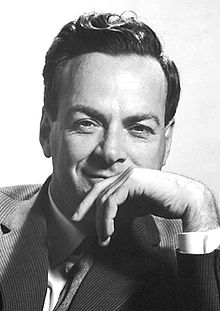
\includegraphics[width=0.8\linewidth]{content/figures/richard_feynman_picuture.jpg}
  \caption{Richard Feynman in 1918\protect\footnotemark}
\end{figure}
\footnotetext{\url{https://upload.wikimedia.org/wikipedia/en/4/42/Richard_Feynman_Nobel.jpg}}

Richard Phillips Feynman (May 11, 1918 – February 15, 1988) was an American theoretical physicist known for his work in the path integral formulation of quantum mechanics, the theory of quantum electrodynamics, and the physics of the superfluidity of supercooled liquid helium, as well as in particle physics for which he proposed the parton model. For his contributions to the development of quantum electrodynamics, Feynman, jointly with Julian Schwinger and Shin'ichiro Tomonaga, received the Nobel Prize in Physics in 1965.

Feynman developed a widely used pictorial representation scheme for the mathematical expressions governing the behavior of subatomic particles, which later became known as Feynman diagrams. During his lifetime, Feynman became one of the best-known scientists in the world. In a 1999 poll of 130 leading physicists worldwide by the British journal Physics World he was ranked as one of the ten greatest physicists of all time.[1]

He assisted in the development of the atomic bomb during World War II and became known to a wide public in the 1980s as a member of the Rogers Commission, the panel that investigated the Space Shuttle Challenger disaster. Along with his work in theoretical physics, Feynman has been credited with pioneering the field of quantum computing and introducing the concept of nanotechnology. He held the Richard C. Tolman professorship in theoretical physics at the California Institute of Technology.

Feynman was a keen popularizer of physics through both books and lectures, including a 1959 talk on top-down nanotechnology called There's Plenty of Room at the Bottom, and the three-volume publication of his undergraduate lectures, The Feynman Lectures on Physics. Feynman also became known through his semi-autobiographical books Surely You're Joking, Mr. Feynman! and What Do You Care What Other People Think? and books written about him, such as Tuva or Bust! and Genius: The Life and Science of Richard Feynman by James Gleick.
